\documentclass{article}

\usepackage[dvipsnames]{xcolor} % Code highlighting color
\usepackage[catalan]{babel} % Language 
\usepackage{indentfirst}
\usepackage{fontspec} 
\usepackage{fullpage}
\usepackage[a4paper, margin=2cm]{geometry} % To change the margins
\usepackage{graphicx} % Insert images
\usepackage[hidelinks]{hyperref} % Links color
\usepackage[final]{pdfpages}
\usepackage{ragged2e}
\usepackage{wrapfig} %To Text wrap
\usepackage{listings} % Add code
\usepackage{verbatim}
\usepackage{nameref}
\usepackage{tikz}
\usepackage{subcaption}
\usepackage{multirow}
\usepackage{colortbl}
\usepackage[backend=bibtex,citestyle=ieee]{biblatex}

\setlength{\parskip}{0.7em}
\setlength{\parindent}{0cm}
\linespread{1.2}

\definecolor{bluekeywords}{rgb}{0.13,0.13,1}
\definecolor{greencomments}{rgb}{0,0.5,0}
\definecolor{redstrings}{rgb}{0.9,0,0}
\lstdefinelanguage{FORTH}
{   
	morekeywords={+, *, -, DO, LOOP, EMIT, DUP, DROP, CR, CHAR, I },
	keywordstyle=\color{bluekeywords},
	sensitive=false,
	basicstyle=\ttfamily,
	breaklines=true,
	xleftmargin=\parindent,
	aboveskip=\bigskipamount,
	tabsize=4,
	morecomment=[l][\color{greencomments}]{\\},
	morecomment=[s][\color{greencomments}]{( }{--\ )},
	morestring=[b]",
	showstringspaces=false,
	stringstyle=\color{redstrings},
}
\lstset{language=FORTH}

\addbibresource{Bibliografia.bib}

\title{
	\Huge
	\textbf{LP} \\ 
	\scshape FORTH
}
\author{
	Joan Marcè i Igual
}
\date{\today}

\begin{document}
\maketitle

\begin{figure}
	\centering
	
\includegraphics[width=0.8\linewidth]{./simple_FIB}
\end{figure}
\newpage

\tableofcontents
\newpage

\section{Introducció}
FORTH va ser dissenyat per \emph{Charles Chuck Moore} \cite{forthEvolution}. Va ser creat als voltants de 1968 orientat a la indústria aeroespacial \cite{nasa} i per ser integrat a aplicacions en temps real per sistemes que no tenien un sistema operatiu molt formal. 

El nom fa referència a que havia de ser la quarta generació de llenguatges\cite{forthGroup} (ve de \emph{fourth} en anglès però la \emph{u} no es va posar perquè el SO utilitzat només suportava 5 caràcters per als noms d'arxius). 

Cap als anys 1980 es va fer força popular ja que era força fàcil de portar a petits computadors de l'època ja que era molt compacte i portable.

\subsection{Influències}

FORTH va ser influenciat pels següents llenguatges de programació \cite{wikipedia}:
\begin{itemize}
	\item Burroughs large systems
	\item Lisp
	\item APL
\end{itemize} 


\section{Principals característiques}
\subsection{Paradigma}

FORTH funciona amb un paradigma \textbf{Imperatiu} i utilitza un \textbf{sistema de pila} per a les operacions. Aquest sistema de pila és diferent al d'altres llenguatges de programació que solen utilitzar-lo pel control de funcions recursives o per emmagatzemar les variables locals de la subrutina, això fa que moltes de les instruccions de FORTH siguin simplement per operar directament amb les dades de la pila.

\subsection{Compilat o interpretat?}

El llenguatge està pensat perquè sigui \textbf{interpretat} tot i que hi ha la opció de compilar certes comandes per a usar-les posteriorment. El sistema funciona de manera que sigui una consola interactiva però si s'han definit fitxers amb tot de paraules(subrutines) del llenguatge aquestes seran compilades per poder-les usar a la consola de FORTH.

\subsection{Comprovació de tipus}

Pel que fa al sistema de tipus hi ha diferents tipus però no es fa comprovació de tipus, és a dir, si el programador s'equivoca al cridar una funció, per exemple si es passa un \emph{float} en lloc de un \emph{int} i es crida la funció \texttt{+} se sumaran els dos valors com si fossin \emph{int} i les dades seran interpretades erròniament. Així que segons els creadors del llenguatge "comprovar els tipus és feina del programador i no de l'interpret".

Així doncs si es volen sumar dos nombres en coma flotant caldrà cridar la funció \texttt{f+}, també hi ha les funcions \texttt{c+, u+} per sumar caràcters i enters sense signe respectivament. D'aquesta manera es pot veure que degut a la no comprovació de tipus tampoc hi ha sobrecàrrega d'operadors. 

\subsection{Sistema de pila} 
Com ja s'ha dit abans, FORTH funciona amb un sistema de pila. Això fa que totes les operacions estiguin orientades al voltant de la pila. 

En el següent exemple a la Figura \ref*{fig:stack_1} es pot veure que s'han inserit els valors \texttt{10} i \texttt{20}. A continuació s'executa la operació \texttt{*} per multiplicar els dos elements que hi ha inserits a la pila (Figura \ref*{fig:stack_2}) i el resultat es guarda a sobre de tot de la pila (els dos elements afegits anteriorment s'han eliminat). S'afegeix el \texttt{50} a la pila (Figura \ref*{fig:stack_3}) i s'executa la operació \texttt{+} (Figura \ref*{fig:stack_4}) obtenint així a sobre de tot de la pila el valor esperat (\texttt{300}).

\begin{lstlisting}[frame=single]
\Exemple per realitzar (25 * 10) + 50
25 10 * 50 +
\end{lstlisting}
\begin{lstlisting}[frame=single,language=TeX]
300 ok
\end{lstlisting}

\begin{figure}[h!]
	\begin{minipage}[b]{0.2\linewidth}
		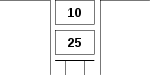
\includegraphics[width=\linewidth]{stack_1}
		\caption{}
		\label{fig:stack_1}
	\end{minipage}
	\hfill
	\begin{minipage}[b]{0.2\linewidth}
		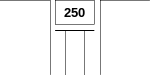
\includegraphics[width=\linewidth]{stack_2}
		\caption{}
		\label{fig:stack_2}
	\end{minipage}
	\hfill
	\begin{minipage}[b]{0.2\linewidth}
		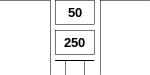
\includegraphics[width=\linewidth]{stack_3}
		\caption{}
		\label{fig:stack_3}
	\end{minipage}
	\hfill
	\begin{minipage}[b]{0.2\linewidth}
		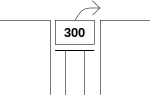
\includegraphics[width=\linewidth]{stack_4}
		\caption{}
		\label{fig:stack_4}
	\end{minipage}
\end{figure}

\section{Exemples}
A continuació es mostren una sèrie d'exemples escrits en FORTH\cite{rosettacode}:

Aquest és l'exemple més bàsic, s'insereix el caràcter "\texttt{*}" a la pila i s'utilitza la comanda \texttt{EMIT} perquè s'imprimeixi per pantalla. També s'està declarant la paraula clau "\texttt{STAR}"
\begin{lstlisting}[frame=single]
: STAR ( -- )           \Imprimeix * per pantalla          
[CHAR] * EMIT ;       	\ $ STAR
						\ *
\end{lstlisting}

En aquest exemple s'utilitza la paraula clau declarada a l'exemple anterior. S'està declarant un bucle que va des de \texttt{0} a \texttt{n-1} (\texttt{n} és un valor que estava inserit a la pila abans de la crida a \texttt{STARS}).
\begin{lstlisting}[frame=single]
: STARS     ( n -- )    \Imprimeix n estrelles
0 DO STAR LOOP        	\Fer n iteracions (de 0 a n-1) i executa
STAR ;                	\ $ 3 STARS
						\ ***
\end{lstlisting}

En aquest exemple també s'utilitza la paraula clau declarada anteriorment tot i que aquí el que s'està fent és posar un bucle dins d'un bucle mitjançant la comanda \texttt{DUP} que duplica el valor de sobre de tot de la pila. Així doncs es duplica \texttt{n} per poder fer un bucle de \texttt{0} a \texttt{n-1} i cridar \texttt{STARS} amb el paràmetre \texttt{n}.
\begin{lstlisting}[frame=single]
: SQUARE    ( n -- )    \Imprimir n^2 estrelles en forma de quadrat
DUP 0 DO              	\ $ 3 SQUARE
DUP STARS CR          	\ ***
LOOP DROP ;           	\ ***
						\ ***
\end{lstlisting}

En aquest exemple s'utilitza la paraula clau \texttt{STARS} per escriure una línia de \texttt{*}. Aquí però també s'utilitza la paraula clau \texttt{I} que permet accedir al comptador dins d'un bucle. Per poder realitzar el bucle correctament aquí primerament s'incrementa en \texttt{1} el valor \texttt{n} que hi havia la pila i es realitza el bucle de \texttt{1} a \texttt{n}.
\begin{lstlisting}[frame=single]
: TRIANGLE  ( n -- )    \Imprimir un triangle de n-línies
1 + 1 DO              	\ $ 3 TRIANGLE
I STARS CR            	\ *
LOOP ;                	\ **
						\ ***
\end{lstlisting}

\section{Llenguatges similars}
A partir de FORTH van aparèixer altres llenguatges que utilitzaven sistemes similars. Un d'ells és el \texttt{RPL} que utilitzen avui dia les calculadores programables HP. També ha inspirat a \emph{PostScript} que s'utilitza en la creació de documents. Altres han estat \emph{Factor o REBOL}.

\printbibliography

\end{document}